\section{21 Nov 23 - Activity: Introduction to Random
Processes}\label{nov-23---activity-introduction-to-random-processes}

So far we have focused on mostly deterministic systems. These are
systems that are typically described by regular ODEs and PDEs; think the
SHO or the Wave Equation. In these systems, the game is to analytically
determine or estimate the trajectory, field, or wave given the set of
equations that describe it. But many processes in nature are random or
have a random element ot them.

How do we model the decay of nuclear isotopes? The gas atoms in a
container? Even things like when your bus will arrive.

Each of these processes has a randomness to it and how we model that
randomness and what we can do depends a lot on the nature of the
randomness. From a mathematical standpoint, what is the distribution of
possible events, or the underlying probability distribution are key
questions to ask in making these models. We will get there, but we will
start by getting intuition from a place you have probably experienced:
rolling dice.

\begin{Shaded}
\begin{Highlighting}[]
\ImportTok{import}\NormalTok{ numpy }\ImportTok{as}\NormalTok{ np}
\ImportTok{import}\NormalTok{ matplotlib.pyplot }\ImportTok{as}\NormalTok{ plt}
\ImportTok{import}\NormalTok{ random }\ImportTok{as}\NormalTok{ rand}
\ImportTok{import}\NormalTok{ numpy }\ImportTok{as}\NormalTok{ np}
\end{Highlighting}
\end{Shaded}

\subsection{The Random Library}\label{the-random-library}

If you have not used \texttt{random}, please read this section because
it has some implementation things that are useful.

Random numbers generated by a computer are not random, so it's important
to know how to use them. They aren't truly random because a computer
must generate them with an algorithm and thus we can potentially
determine every number we'd receive if we knew the algorithm. There's
tons of research into how to generate good random numbers and there's
precious few ways. The main way right now is the
\href{https://en.wikipedia.org/wiki/Mersenne_Twister}{Mersenne Twister
method}. Testing the quality of a random number generator is beyond the
scope of this class, but a useful exercise if you are doing research
into random processes.

\subsubsection{Seeding the number
generator}\label{seeding-the-number-generator}

But because it's an algorithm, we can control the sequence of random
numbers we get. That is we can tell the random number generator to
create random numbers for us in the same way. This helps because we can
use them and test them over and over before running a full simulation.
See below on how to generate random integers. Re-run to observe what
happens.

\begin{Shaded}
\begin{Highlighting}[]
\NormalTok{start }\OperatorTok{=} \DecValTok{1}
\NormalTok{stop }\OperatorTok{=} \DecValTok{10}

\NormalTok{a }\OperatorTok{=}\NormalTok{ rand.randint(start,stop)}
\BuiltInTok{print}\NormalTok{(}\StringTok{\textquotesingle{}a =\textquotesingle{}}\NormalTok{, a)}
\NormalTok{rand.seed(}\DecValTok{42}\NormalTok{)}
\NormalTok{b }\OperatorTok{=}\NormalTok{ rand.randint(start,stop)}
\BuiltInTok{print}\NormalTok{(}\StringTok{\textquotesingle{}b =\textquotesingle{}}\NormalTok{, b)}
\NormalTok{rand.seed(}\DecValTok{18}\NormalTok{)}
\NormalTok{c }\OperatorTok{=}\NormalTok{ rand.randint(start,stop)}
\BuiltInTok{print}\NormalTok{(}\StringTok{\textquotesingle{}c =\textquotesingle{}}\NormalTok{, c)}
\NormalTok{rand.seed(}\DecValTok{42}\NormalTok{)}
\NormalTok{d }\OperatorTok{=}\NormalTok{ rand.randint(start,stop)}
\BuiltInTok{print}\NormalTok{(}\StringTok{\textquotesingle{}d =\textquotesingle{}}\NormalTok{, d)}
\end{Highlighting}
\end{Shaded}

\begin{verbatim}
a = 5
b = 2
c = 3
d = 2
\end{verbatim}

\subsection{Creating a uniform
distribution}\label{creating-a-uniform-distribution}

One of the simplest distributions to generate is one that you are likely
most familiar with - a fair die or pair of dice. In the case of a single
fair die, each outcome is equally likely and distinct from each other.
That is rolling a one and rolling a six are different, distinct outcomes
- and we can say that for each outcome.

Below, write a short piece of code (maybe as a function), that rolls one
N-sided die as many times as you like and returns all the outcomes.
\textbf{Be careful using rand.seed() here because you can just an array
of all the same numbers!}

Plot a histogram of the outcomes; vary the sides of the die and the
number of times it rolls.

\textbf{Can you come up with a scheme that quantifies how close your
distribution is to uniform?}

\begin{Shaded}
\begin{Highlighting}[]
\CommentTok{\#\# your code here}
\end{Highlighting}
\end{Shaded}

\subsubsection{Make a biased die}\label{make-a-biased-die}

Adjust your program so that you get even numbered rolls twice as
frequently as odd rolls. This is the basis for baking in a probability
function into our models. So do try to this. \textbf{Make a histogram of
the results of the biased die}

\begin{Shaded}
\begin{Highlighting}[]
\CommentTok{\#\# Your code here}
\end{Highlighting}
\end{Shaded}

\subsubsection{Micro vs Macro states}\label{micro-vs-macro-states}

In many random processes, the results are not distinct. Think about
rolling two dice (colors are green and white) instead. How many ways can
you get a sum of 2 vs a sum of 6? The state of the two dice where we
indicate the number of each die can be called a ``microstate''. The
state of the sum can be called a ``macrostate.''

So as an example consider the macrostate with a sum of 4. This can be
constructed of out 3 potential microstates. First the green die could
have a 1 and the white one a 3, the green could have a 2 and the white a
2, and then the green could have a 3 and the white a 1. But the result I
care about is not the individual die, but the sum. Regardless I get 4.

\begin{itemize}
\tightlist
\item
  Microstate - tracks individual constituent states as if they were
  unique
\item
  Macrostate - a group of microstates that share something
\end{itemize}

\textbf{Modify or use your code above to roll two fair die and count
their sum}

Plot the resulting histogram of macrostates. Vary the number of sides
and number of rolls. What do you notice?

\begin{Shaded}
\begin{Highlighting}[]
\CommentTok{\#\# your code here}
\end{Highlighting}
\end{Shaded}

\subsection{Poisson Processes}\label{poisson-processes}

Many events in physics can be represented by a
\href{https://en.wikipedia.org/wiki/Poisson_distribution}{Poisson
Distribution}, which results from events that have the following
properties:

\begin{itemize}
\tightlist
\item
  The occurrence of one event does not affect the probability that a
  second event will occur. That is, events occur independently.
\item
  The average rate at which events occur is independent of any
  occurrences. For simplicity, this is usually assumed to be constant,
  but may in practice vary with time.
\item
  Two events cannot occur at exactly the same instant; instead, at each
  very small sub-interval, either exactly one event occurs, or no event
  occurs.
\end{itemize}

Oftentimes, it's the average rate (think lifetime of an isotope) that we
think about as helping us decide. If it's true that the rate is roughly
constant and the events are independent, then this modeling can work
reasonably well. So an event can be random, but the average result
should be relatively simple (e.g., a single average decay time), then we
can consider the events Poisson distributed.

\subsubsection{Decay of an isotope}\label{decay-of-an-isotope}

Consider a collection of \(^{208}Tl\) that decays into \(^{208}Pb\) with
a half-life of 3.053 minutes. Note that any one atom decays randomly at
a random time, but on average, we see that \(1/e\) atoms decay in 3.053
minutes (this is characteristic of a Poisson Process).

The number of atoms \(N\) that will remain in our sample (that is still
be Thallium 208) will fall off exponentially over time (we could observe
that from data):

\[N(t) = N(0)2^{-t/\tau}\]

where \(\tau\) is the half-life. The fraction of remaining Thallium 208
atoms at any given time \(t\) is:

\[\dfrac{N(t)}{N(0)} = 2^{-t/\tau}\]

The probability that an atom decayed into Lead 208 is just this number
subtracted from one:

\[p(t) = 1 - 2^{-t/\tau}\]

\begin{Shaded}
\begin{Highlighting}[]
\CommentTok{\# Constants}
\NormalTok{NTl }\OperatorTok{=} \DecValTok{1000}          \CommentTok{\# Starting Thallium Atoms}
\NormalTok{NPb }\OperatorTok{=} \DecValTok{0}             \CommentTok{\# Starting Lead Atoms}
\NormalTok{tau }\OperatorTok{=} \FloatTok{3.053}\OperatorTok{*}\DecValTok{60}      \CommentTok{\# Half life in seconds}
\NormalTok{h }\OperatorTok{=} \FloatTok{1.0}             \CommentTok{\# Time step between checking if a decay occurred}
\NormalTok{p }\OperatorTok{=} \DecValTok{1} \OperatorTok{{-}} \DecValTok{2}\OperatorTok{**}\NormalTok{(}\OperatorTok{{-}}\NormalTok{h}\OperatorTok{/}\NormalTok{tau) }\CommentTok{\# Probability the decay occurs in that time elapsed}
\NormalTok{tmax }\OperatorTok{=} \DecValTok{1000}         \CommentTok{\# Total time in seconds }

\CommentTok{\# List of plot points}
\NormalTok{tpoints }\OperatorTok{=}\NormalTok{ np.arange(}\FloatTok{0.0}\NormalTok{, tmax, h)}
\NormalTok{Tlpoints }\OperatorTok{=}\NormalTok{ []}
\NormalTok{Pbpoints }\OperatorTok{=}\NormalTok{ []}
\NormalTok{probabilities }\OperatorTok{=}\NormalTok{ []}

\CommentTok{\# Model}
\ControlFlowTok{for}\NormalTok{ t }\KeywordTok{in}\NormalTok{ tpoints:}
    
\NormalTok{    Tlpoints.append(NTl)}
\NormalTok{    Pbpoints.append(NPb)}
    
    \CommentTok{\#\# Calculate the number of atoms that decay}
\NormalTok{    decay }\OperatorTok{=} \DecValTok{0}
    \ControlFlowTok{for}\NormalTok{ i }\KeywordTok{in} \BuiltInTok{range}\NormalTok{(NTl):        }\CommentTok{\# For each atom in the sample}
        \ControlFlowTok{if}\NormalTok{ rand.random() }\OperatorTok{\textless{}}\NormalTok{ p:   }\CommentTok{\# Check if it decayed in the last dt }
\NormalTok{            decay }\OperatorTok{+=} \DecValTok{1}
\NormalTok{    NTl }\OperatorTok{{-}=}\NormalTok{ decay}
\NormalTok{    NPb }\OperatorTok{+=}\NormalTok{ decay}

\CommentTok{\# Plot the data}
\NormalTok{plt.figure(figsize}\OperatorTok{=}\NormalTok{(}\DecValTok{8}\NormalTok{,}\DecValTok{6}\NormalTok{))}
\NormalTok{plt.plot(tpoints, Tlpoints, label}\OperatorTok{=}\VerbatimStringTok{r\textquotesingle{}}\DecValTok{$\^{}}\OperatorTok{\{208\}}\VerbatimStringTok{Tl}\DecValTok{$}\VerbatimStringTok{\textquotesingle{}}\NormalTok{)}
\NormalTok{plt.plot(tpoints, Pbpoints, label}\OperatorTok{=}\VerbatimStringTok{r\textquotesingle{}}\DecValTok{$\^{}}\OperatorTok{\{208\}}\VerbatimStringTok{Pb}\DecValTok{$}\VerbatimStringTok{\textquotesingle{}}\NormalTok{)}
\NormalTok{plt.xlabel(}\StringTok{\textquotesingle{}Time (s)\textquotesingle{}}\NormalTok{)}
\NormalTok{plt.ylabel(}\StringTok{\textquotesingle{}Number of atoms\textquotesingle{}}\NormalTok{)}
\NormalTok{plt.legend()}
\NormalTok{plt.grid()}
\end{Highlighting}
\end{Shaded}

\begin{figure}
\centering
\pandocbounded{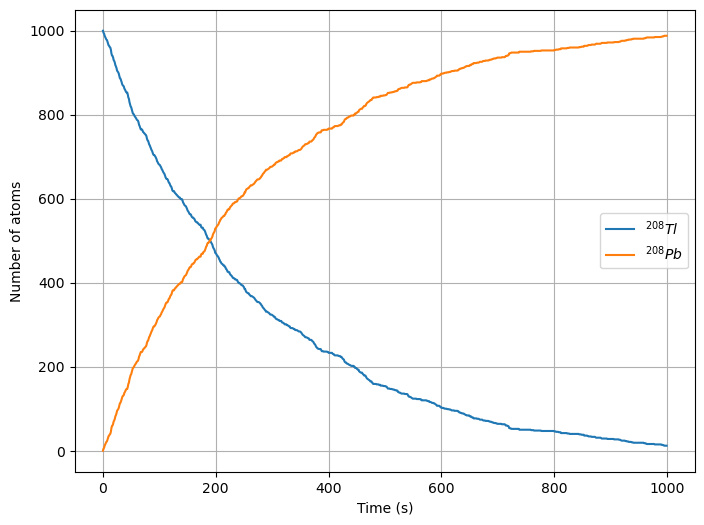
\includegraphics[keepaspectratio,alt={png}]{../images/activity-radioactive_decay_activity-radioactive_decay_tmp_12_0.png}}
\caption{png}
\end{figure}

\subsubsection{Decay Chains}\label{decay-chains}

Here's the big project for today! It is less often the case that decays
happen like above. Many times there are {[}Decay Channels{]} where the
atoms decay over time into different elements with different
probabilities. Consider the Bismuth 213 decay to Bismuth 209. It decays
in two channels:

\[^{213}Bi \rightarrow  ^{209}Tl \rightarrow  ^{209}Pb \rightarrow  ^{209}Bi\]
\[^{213}Bi \rightarrow  ^{209}Pb \rightarrow  ^{209}Bi\]

The first channel happens to about 2.09\% of atoms. So we will ignore it
for now. Let's focus on the two step decay to Lead.

Rewrite the model above to account for both decays, which have lifetimes
of 46 minutes (\(^{213}Bi \rightarrow ^{209}Pb\)) and 3.3 hours
(\(^{209}Pb \rightarrow  ^{209}Bi\)) respectively.

\textbf{Plot the number of all three atoms as a function of time}

\begin{Shaded}
\begin{Highlighting}[]
\CommentTok{\#\# Your code here}
\end{Highlighting}
\end{Shaded}

\subsubsection{A Challenge}\label{a-challenge}

Model the entire decay including the random but clearly biased split
between Lead 209 and Thallium 209, which has a halflife of 2.2 minutes.

\emph{Note: We are not including the transition between Bismuth 213 and
Polonium 209, which is a very short lived isotope.}

\textbf{Plot the number of all four atoms as a function of time}

\begin{Shaded}
\begin{Highlighting}[]
\CommentTok{\#\# Your code here}
\end{Highlighting}
\end{Shaded}
